% REMEMBER TO SET LANGUAGE!
\documentclass[a4paper,10pt,English]{article}
\usepackage[utf8]{inputenc}
\usepackage[citestyle=alphabetic,bibstyle=authortitle]{biblatex}
\bibliography{project1_refs.bib}
\usepackage[options ]{algorithm2e}
% Standard stuff
\usepackage{amsmath,graphicx,varioref,verbatim,amsfonts,geometry}
% colors in text
\usepackage{xcolor}
% Hyper refs
\usepackage[colorlinks]{hyperref}

% Document formatting
\setlength{\parindent}{0mm}
\setlength{\parskip}{1.5mm}

%Color scheme for listings
\usepackage{textcomp}
\definecolor{listinggray}{gray}{0.9}
\definecolor{lbcolor}{rgb}{0.9,0.9,0.9}

%Listings configuration
\usepackage{listings}
%Hvis du bruker noe annet enn python, endre det her for å få riktig highlighting.
\lstset{
	backgroundcolor=\color{lbcolor},
	tabsize=4,
	rulecolor=,
	language=python,
        basicstyle=\scriptsize,
        upquote=true,
        aboveskip={1.5\baselineskip},
        columns=fixed,
	numbers=left,
        showstringspaces=false,
        extendedchars=true,
        breaklines=true,
        prebreak = \raisebox{0ex}[0ex][0ex]{\ensuremath{\hookleftarrow}},
        frame=single,
        showtabs=false,
        showspaces=false,
        showstringspaces=false,
        identifierstyle=\ttfamily,
        keywordstyle=\color[rgb]{0,0,1},
        commentstyle=\color[rgb]{0.133,0.545,0.133},
        stringstyle=\color[rgb]{0.627,0.126,0.941}
}


%opening
\title{A Study of a Numerical Approximation to the Poisson Equation using Linear Algebra}
\author{Caspar William Bruenech}

\begin{document}

\maketitle

\begin{abstract}
    In this experiment the one-dimensional Poisson equation was solved using different linear algebra methods. By rewriting the equation as a matrix-vector multiplication, a tridiagonal matrix with constant values was produced. A general algorithm for solving the equation with a tridiagonal matrix was used to solve the equation, in addition to a specialized algorithm taking advantage of the constant values in the matrix. Both algorithms produced similar results, while showing a significant difference in the CPU time used for higher matrix sizes. The specialized algorithm performed twice as fast as the general, which was in line with the theoretically calculated floating point operations. The algorithms were also compared with an lu-decomposition, which performed between $500$ and $1000$ times slower than the algorithms, which was also to be expected from the complexity model of the Lu-factorization algorithm. Finally, loss of numerical precision was witnessed to produce great errors in the approximations as the resolution of the data reached a value exceeding $10^5$ data points. The result show a clear advantage for tridiagonal matrices when solving systems of linear equations while exemplifying the problems of machine numbers.
\end{abstract}

\section{Introduction}

\subsection{The Poisson Equation}
In this project we will look at different numerical methods for various vector and matrix operations. We will also compare different algorithms for solving a set of linear equations by observing the CPU time for each algorithm. Finally we will look at how loss of numerical precision can lead to big errors. The case we will study is Poisson's equation from electromagnetism:

\begin{equation}
    \nabla^2 \Phi = -4\pi \rho(\vec{r})
\end{equation}

Assuming a spherically symmetrical $\Phi$ and $\rho(\vec{r})$, and using substitution, we can rewrite this as:

\begin{equation}
    \frac{d^2 \phi}{dr^2} = -4\pi r \rho(r)
\end{equation}

Finally, by limiting ourselves to the one-dimensional case, we get the general one-dimensional Poisson equation:

\begin{equation}\label{eq:poisson}
    -u''(x) = f(x)
\end{equation}

This is the equation we want to solve, with the addition of Dirichlet boundary conditions. I.e. we want to solve:

$$-u''(x) = f(x) \qquad x \in (0, 1) \qquad u(0) = u(1) = 0$$

By using the approximation of the double derivative, we can discretize this equation:

\begin{equation} \label{eq: poi_disc}
    -\frac{v_{i+1} + v_{i-1} - 2v_i}{h^2} = f_i \qquad \text{for}  \quad i = 1,....,n
\end{equation}

Where $v_i = u(x_i)$, $f_i = f(x_i)$. Here we have defined $x = ih$ where $h$ is the step length defined as $h = \frac{1}{n+1}$.

\subsection{A Linear Equation}

By multiplying both sides with $h^2$, and defining $d_i = h^2 f_i$ we get:

$$-v_{i-1} + 2v_i - v_{i+1} = d_i$$

Which gives us the equations:

$$ 2v_0 - v_1 = d_0 $$
$$-v_0 + 2v_1 - v_2 = d_1$$

$$ \vdots $$

$$  -v_{n-1} + 2v_n = d_n$$

We recognize this as a set of linear equations, which as we know can be written as a matrix-vector multiplication. By creating $\vec{v} = \begin{bmatrix} v_0 \\ v_2 \\ \vdots \\ v_n \end{bmatrix}$ and $\vec{d} = \begin{bmatrix} d_0 \\ d_1 \\ \vdots \\ d_n \end{bmatrix}$ we see that we can write this as $A\vec{v} = \vec{d}$ where 

$$A = \begin{bmatrix}
2 & -1 & 0 & \dots & \dots & 0 \\
-1 & 2 & -1 & 0 & \dots & \dots \\
0 & -1 & 2 & -1 & 0 & \dots \\
\vdots & \dots & \dots & \dots & \dots & \dots \\
0 & \dots & \dots & -1 & 2 & -1 \\
0 & \dots & \dots & 0 & -1 & 2 
\end{bmatrix}
$$

In this project we will set the source term as $f(x) = 100e^{-10x}$ which gives us $d_i = 100h^2 e^{-10*x_i}$, and which has an analytical solution to \ref{eq:poisson} as:

\begin{equation}\label{eq:exact}
    u(x) = 1 - (1 - e^{-10})x - e^{-10x}
\end{equation}

To prove this, we can simply insert it into \ref{eq:poisson}. We can do this by finding the second derivative:

$$u'(x) = 10 e^{-10x} - 1 + \frac{1}{e^10}$$

$$u''(x) = -100e^{-10x} = -f(x)$$

\section{Method}

\subsection{The general case} \label{sec:general}
Our first objective is to create a general algorithm for solving the matrix-vector multiplication in which the matrix A does \textit{not} necessarily have identical values along the upper, lower, and diagonal elements. I.e. we want to design an algorithm that solves for $\vec{v}$ :

\begin{equation}
    \begin{bmatrix}
b_1 & c_1 & 0 & \dots & \dots & 0 \\
a_1 & b_2 & c_2 & 0 & \dots & \dots \\
0 & a_2 & b_3 & c_3 & 0 & \dots \\
\vdots & \dots & \dots & \dots & \dots & \dots \\
0 & \dots & \dots & a_{n-2} & b_{n-1} & c_{n-1} \\
0 & \dots & \dots & 0 & a_{n-1} & b_n 
\end{bmatrix} \begin{bmatrix} v_1 \\ v_2 \\ \vdots \\ v_n \end{bmatrix} = \begin{bmatrix} d_1 \\ d_2 \\ \vdots \\ d_n \end{bmatrix}
\end{equation}

To do this, we can start with the brute-force Gaussian Elimination method. This will consist of two steps: (1) Forward substitution: getting all the elements under the diagonal to equal zero, and (2) backward substitution, calculating each value of $v_i$ by inserting $v_{i+1}$. We see that we can get $a_i = 0$ by subtracting $\frac{b_{i-1}}{b_{i-1}}*a_i$ from $a_i$. This means we have to subtract $a_i \times R_{i-1}$ from $R_i$, where $R_i$ denotes row $i$ in A. The resulting algorithm is a specialized case of Gaussian elimination for a tridiagonal matrix, and is named the Thomas Algorithm, after Llewellyn Thomas \cite{Thomas1949}:
\begin{align}
    
\begin{algorithm}[H]
\SetAlgoLined
\textbf{Forward substitution}

 \For{i = 2,...,n}{
  b_i = b_i - a_i * c_{i-1}/b_{i-1}\\
  d_i = d_i - a_i*d_{i-1}/b_{i-1}\\
  }
\textbf{Backward substitution}\\
    v_n = d_n/b_n\\
    \For{i = n-1,...,1}{
    v_i = (d_i - c_i*v_{i+1})/b_i\\
 }
 \caption{Thomas algorithm}

\end{algorithm}
\end{align}


\subsection{The special case} \label{sec:spec}

The next task is to specialize the above algorithm to the case at hand in which the upper and lower diagonal elements are constant and identical, and the diagonal elements are constant. By simply inserting the values into the algorithm we get:


\begin{algorithm}[H]
\SetAlgoLined
\textbf{Forward substitution}

 \For{i = 2,...,n}{
  b_i = b_i - (-1)*(-1)/b_{i-1} = b_i - \frac{1}{b_{i-1}}\\
  d_i = d_i - (-1)*d_{i-1}/b_{i-1} ) = d_i + \frac{d_{i-1}}{b_{i-1}}\\
  }
\textbf{Backward substitution}\\
    v_n = d_n/b_n\\
    \For{i = n-1,...,1}{
    v_i = \frac{d_i - (-1)*v_{i+1}}{b_i} = \frac{d_i + v_{i+1}}{b_i}\\
 }
 \caption{Specialized Thomas algorithm}

\end{algorithm}


\section{Implementation}

All the relevant programs, including figures and benchmarks, can be found in the following github repository:

\begin{center}
    \url{https://github.com/casparwb/FYS3150/tree/master/1_project}
\end{center}

\begin{figure}
    \centering
    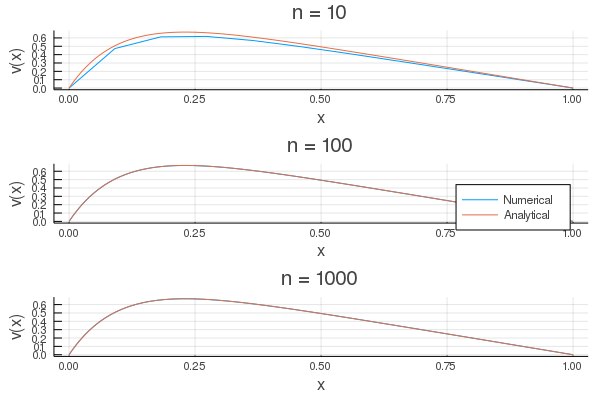
\includegraphics[width = 0.8\textwidth]{1bplot.png}
    \caption{A plot showing the analytical vs the numerical solution of the Poisson equation with varying number of grid points. The numerical values were calculated using the general Thomas Algorithm.}
    \label{fig:1b}
\end{figure}

Figure \ref{fig:1b} shows three plots of the analytical versus the numerical solution (calculated with the general algorithm) to the differential equation, with an increasing number of grid points, 

\begin{table}[] \label{tab: CPU_t} \centering
\begin{tabular}{|l|l|l|l|}
\hline
\textbf{\#$log_{10} n$} & \textbf{General time (ms)} & \textbf{Specialized time (ms)} & \textbf{$t_{gen}/t_{spec}$} \\ \hline
1                       & 0.000270                    &  0.000170                         & 1.589                       \\ \hline
2                       & 0.002200                     & 0.001090                         & 2.018                       \\ \hline
3                       & 0.020940                     & 0.010730                         & 1.951                       \\ \hline
4                       & 0.202759                     & 0.099850                         & 2.030                       \\ \hline
5                       & 1.976950                     & 0.975680                         & 2.026                       \\ \hline
6                       & 20.332870                   & 10.055740                        & 2.022                       \\ \hline
\end{tabular}
\caption{A table showing the CPU times of the general and specialized algorithm with number of grid points up to $10^6$. Each time measurement is an average of 10 functions calls for each value of $n$.}
\end{table}

while table \ref{tab: CPU_t} shows the CPU time of both the general and special algorithm with grid points up to $10^6$.

\begin{figure}
    \centering
    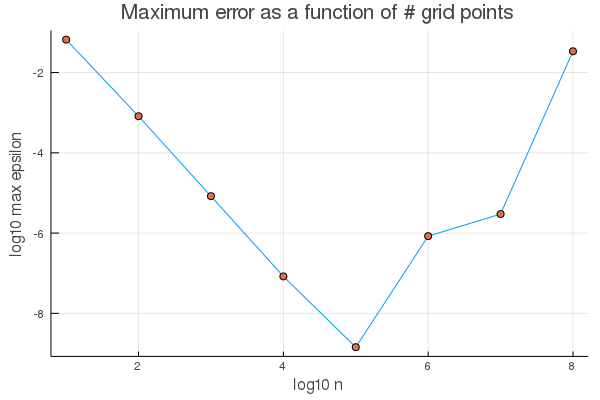
\includegraphics[width=0.7\textwidth]{max_error.png}
    \caption{A plot showing the maximum error as a function of # grid points. Each dot is the maximum value of \ref{eq:epsilon} for each corresponding value of n.}
    \label{fig:epsilon}
\end{figure}

To compute the relative error of the data set, the function

\begin{equation}\label{eq:epsilon}
    \epsilon_i = \log_{10} \left( \vleft \frac{v_i - u_i}{u_i} \vright \right)
\end{equation}

was set up. The numerical values produced by the general algorithm was then inserted, along with the exact values from the analytical expression. Finally, the maximum value of \ref{eq:epsilon} was extracted. The result is shown in figure \ref{fig:epsilon}. We see that the maximum error decreases linearly until $n=10^5$. As $n$ is further increased to $10^6$, the error is also increased, and rises proportional to $n$.

Finally, the CPU time of the two implemented algorithms was compared to LU-decomposition using a built-in function in the Julia language's Linear Algebra package. The result it shown in table \ref{tab:LU}. 


\begin{table}[] \label{tab:LU} \centering
\begin{tabular}{|l|l|l|l|}
\hline
$log_{10} n$ & General time (ms) & Specialized time (ms) & LU decomp. time (ms) \\ \hline
1            & 0.000270            & 0.000170                & 0.004070               \\ \hline
2            & 0.002200            & 0.001090                & 3.909450               \\ \hline
3            & 0.020940            & 0.010730                & 28.698900              \\ \hline
\end{tabular}
\caption{An overview of the CPU time of the general and special algorithm compared to the CPU time of LU decomposition on a matrix with size $n\times x$. Each time measurement is an average of 10 functions calls for each value of $n$.}
\end{table}
\section{Analysis}

Figure \ref{fig:1b} shows that the the two solutions are visually distinguishable at $n = 10$ grid points, but at $n = 100$ and $n = 1000$ it is harder to see a difference between the approximated values and the analytical, meaning that the accuracy increases as the step length $h$ decreases. This is because of our approximation of the second derivative. Since the true derivative is defined as;

$$u''(x) = \lim_{h \to \infty} \frac{u(x-h) - 2u(x) + u(x + h)}{h^2}$$

and our $h$ is not an infinitesimal value, the approximation of $u''(x)$ also carries an error term $O(h)$ which goes as (\cite{Hjorth-Jensen2015}):

$$O_i(h) = 2 \sum_{j = i}^\infty \frac{h^{2j} v_i^{(2j+2)}}{(2j+1)!}$$

where $O_i$ is the error for the approximated value $v_i$ and $v_i^{(2j+2)}$ is the $(2j+2)$-th derivative of $v_i$. Since $h < 1$, we see that the error should decrease as the number of grid points increases, which is also what we see in the figure. 

\newline

The data in table \ref{tab: CPU_t} tells us that the speed of the specialized algorithm approaches twice the speed of the general as $n$ is increased, while performing around $50\%$ faster for $n < 10^3$. To analyse this, we need to look at the number of flops in each algorithm. Assuming each mathematical operation requires the same amount of computing power (in reality this is not true), we can count the total number of flops as the sum of all additions, subtractions, multiplications and divisions. For the forward substitution loop which runs a total of $n-1$ times, we have 2 subtractions, 2 multiplication, and two divisions, for a total of $6(n-1)$ flops. For the backward substitution, we first have one division, followed by a loop which has $n$ iterations, each with one division, one multiplication, and one division, which gives us $1 + 3n$ flops. The total amount of flops is then 

$$flops_{gen} = 6(n-1) + 1 + 3n = 9n - 5$$

We can perform the same counting for the special algorithm. In this case, we have $2\times 2$ flops in each iteration of the forward substitution loop, followed by one division and $2$ operation in each iteration of the backward substitution loop. This gives us:

$$flops_{spec} = 4(n-1) + 1 + 2n = 6n - 3$$

In fact, this specialised algorithm has an analytical expression for the diagonal values $b_i$ \cite{Hjorth-Jensen2015}, given as:

$$b_i = \frac{i+1}{i}$$

Knowing this, we can precalculate the $b_i$-values, and reduce the number of flops to actually be $4n - 3$. We see that while both algorithms have a complexity of $O(n)$, the specialized algorithm has a slightly lower slope than the specialized, which means the computation time will increase slightly less than with the general algorithm as $n$ is increased.

\begin{figure}
    \centering
    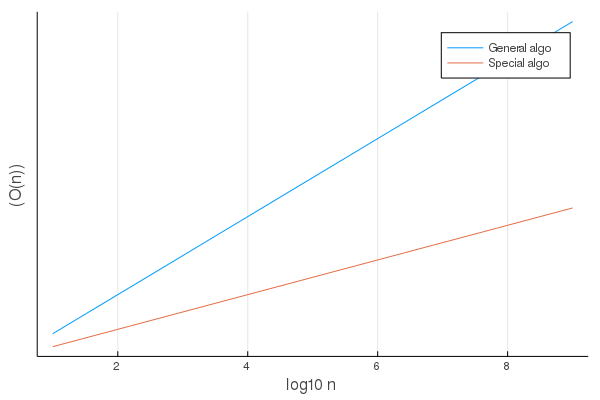
\includegraphics[width=0.8\textwidth]{o(n).png}
    \caption{A plot showing the number of floating point operations for each of the two algorithm as a function of number of grid points.}
    \label{fig:complexity}
\end{figure}

This is shown in figure \ref{fig:complexity}. As we see, the two lines are closer for lower values of $n$, which explains the low relative difference between the CPU time of both algorithm for $n \leq 10^2$.

\newline

The relative maximum error (as shown in figure \ref{fig:epsilon}) was calculated using the general algorithm. The figure shows that the error decreases as $n$ increases. A higher $n$ implies a smaller $h$, which as we already mentioned, decreases the error. However, as $n$ becomes higher than $10^5$, the error starts increasing again. The reason for this is the limited precision in numerical numbers. A floating point number is stored in a computer as an approximation of the real number (part 1, chap. 2.3.2 of \cite{Hjorth-Jensen2015}). As $n$ increases, $h$ becomes smaller, and the difference between each of the values in the arrays also decreases. This means that as we calculate the next value, which is dependent on the previous value, we are subtracting two very similar numbers and then dividing by this sum. As seen in \cite{Hjorth-Jensen2015}, the error in the resulting product, when $b \approx c$, is given as:

$$\epsilon_a \approx \frac{b}{a} (\epsilon_b - \epsilon-c)$$

where $b$ and $c$ are the two similar number who are being subtracted. When $a$ is small, which it is when $n$ is large, the error can become very large, which is exactly what we see in figure \ref{fig:epsilon}.

\newline

To compare the CPU time of the two algorithms with the CPU time of an LU decomposition, a full matrix was constructed and LU-factorized using a function in the Linear Algebra package for Julia (see \footnote{\url{https://docs.julialang.org/en/v1/stdlib/LinearAlgebra/index.html}} for documentation). Running this for $n = 10, 100, 1000$, the results are shown in table \ref{tab:LU}. We see that for $n=10$, the CPU time of the LU-decomposition is already around 20 times slower than the average of the general and the specialized algorithm. However, as $n$ is increased by a factor of $10$, the time used is increased by a factor of $960$, compared to $8.15$ and $6.41$ for respectively the general and specialized algorithm. The reason for this is is how the complexity of the LU factorization scales. As we saw earlier, the two algorithms both scales with $n$. However, an LU decomposition scales as $\frac{2}{3}n^3$ \cite{Golub1996}. Notice that $960 > \frac{2}{3}10^3 = 667$. This may be attributed to a combination of the granularity of the timer, and memory reads and writes, which are not accounted for in the complexity model. Still, not only is the CPU time significantly higher than for the Thomas algorithms, but when performing this factorization, we also apply it to a full matrix. With tridiagonal matrices, we only need to store the lower, upper, and diagonal elements as individual arrays, significantly reducing the amount of data that needs to be looped over, compared to a dense matrix. This fact also leads to another issue, as when trying to run the LU-factorization with a matrix of size $10^5 \times 10^5$, an error is returned, stating that the program has run out of memory. This means that the byte size of the matrix is larger than the memory available. While this is dependent on the hardware available, there is no doubt that having to store an entire matrix compared to three arrays will have an impact on the program. For example, with the stated size of $n=10^5$, the Thomas algorithm has to allocate a total of $5$ arrays each with a size of $n$, which, when using double-precision, equals a total of $5*10^5*8bytes = 4 \times 10^6 bytes = 4mb$. The specialized algorithm has to allocate even less, with only $3$ arrays necessary, totaling $2.4mb$. For a full matrix of size $n \times n$, the allocated memory is equal to $10^{10}*8bytes = 8gb$. The program in this report was run on hardware with $8gb$ of RAM, which is why it was not able to perform an LU factorization of a matrix of this size. It should be noted that it is possible to perform the factorization with matrices of larger size than the available memory, but this will significantly slow down the program, as data will be stored in virtual memory, where reading and writing is significantly slower.


\section{Conclusion}


In conclusion, it is apparent that having a tridiagonal matrix when solving a matrix-vector multiplication is favourable to having a dense matrix. While a normal matrix factorization scales with its size cubed, a tridiagonal matrix scales (theoretically) linearly with its size, and, as we have seen, with an even shallower slope for a tridiagonal matrix with constant values. At the same time, the amount of memory needed to allocate for storing the values in the matrix is vastly reduced for a tridiagonal matrix, as only three one-dimensional vectors are required. This can also impact the calculation time, as the size of the matrix can easily exceed the available memory of the hardware (this of course depends on the hardware, but even for hardware with large memory, the processor cache is usually small). We have also seen how the limited accuracy in machine numbers can lead to loss of numerical precision when the elements in a mathematical operations become too small. In this specific project we saw that when we wanted a higher resolution in our approximated solution, the size of the matrix and vectors was increased, which caused the difference in values between each successive element to become small. At $n=10^6$, this difference was small enough such that the error in the machine numbers was no longer insignificant, causing the solution to produce an error which only increased as more values were computed, resulting in a higher maximum error, as seen in figure \ref{fig:epsilon}. While we obviously want to produce results with as high an accuracy as possible, it is important to be aware of the limited accuracy of computers, and how this can lead to loss of numerical precision, which again can cause a domino effect, resulting in large errors in the computed approximations. 


\section*{Notes}

When timing calculations, there is always a certain amount of variation for each run of the program. This is especially present when performing calculations as small as the ones in this experiment. Despite doing an average of the CPU time of 10 function calls, the times varied with about $\Delta \frac{t_{gen}}{t_{spec}} \approx 0.5$. However, the results still paint a clear picture of the main ideas presented in this paper.

\printbibheading
\printbibliography




\end{document}
